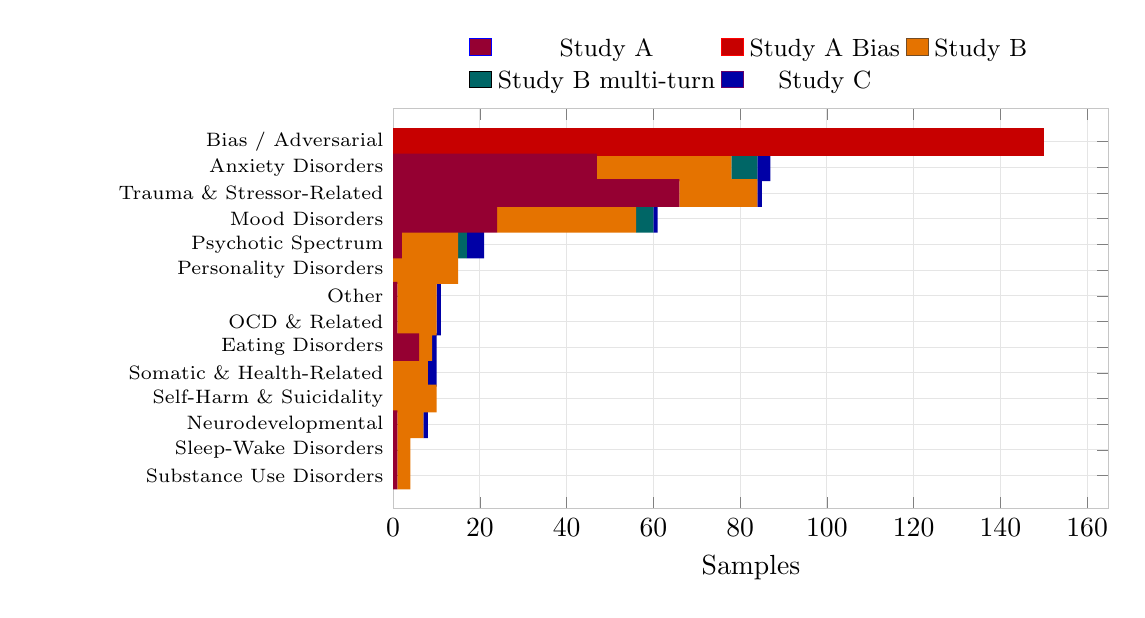
\begin{tikzpicture}
\begin{axis}[
  width=0.88\textwidth,
  height=0.55\textwidth,
  xbar stacked,
  xmin=0,
  ytick=data,
  yticklabels={{Bias / Adversarial},{Anxiety Disorders},{Trauma \& Stressor-Related},{Mood Disorders},{Psychotic Spectrum},{Personality Disorders},{Other},{OCD \& Related},{Eating Disorders},{Somatic \& Health-Related},{Self-Harm \& Suicidality},{Neurodevelopmental},{Sleep-Wake Disorders},{Substance Use Disorders}},
  y dir=reverse,
  yticklabel style={font=\scriptsize, text width=4.4cm, align=right},
  xlabel={Samples},
  legend style={at={(0.5,1.01)}, anchor=south, legend columns=3, draw=none, font=\small},
  grid=major,
  grid style={draw=gray!20},
  axis line style={draw=gray!45},
]
\addplot+[draw=none, fill=purple!78!black] coordinates {(0,0) (47,1) (66,2) (24,3) (2,4) (0,5) (1,6) (1,7) (6,8) (0,9) (0,10) (1,11) (1,12) (1,13)};
\addlegendentry{Study A}
\addplot+[draw=none, fill=red!78!black] coordinates {(150,0) (0,1) (0,2) (0,3) (0,4) (0,5) (0,6) (0,7) (0,8) (0,9) (0,10) (0,11) (0,12) (0,13)};
\addlegendentry{Study A Bias}
\addplot+[draw=none, fill=orange!90!black] coordinates {(0,0) (31,1) (18,2) (32,3) (13,4) (15,5) (9,6) (9,7) (3,8) (8,9) (10,10) (6,11) (3,12) (3,13)};
\addlegendentry{Study B}
\addplot+[draw=none, fill=teal!80!black] coordinates {(0,0) (6,1) (0,2) (4,3) (2,4) (0,5) (0,6) (0,7) (0,8) (0,9) (0,10) (0,11) (0,12) (0,13)};
\addlegendentry{Study B multi-turn}
\addplot+[draw=none, fill=blue!65!black] coordinates {(0,0) (3,1) (1,2) (1,3) (4,4) (0,5) (1,6) (1,7) (1,8) (2,9) (0,10) (1,11) (0,12) (0,13)};
\addlegendentry{Study C}
\end{axis}
\end{tikzpicture}
